% !TeX spellcheck = en_US
\documentclass[./main.tex]{subfiles}
\begin{document}

\section{Relevant links}

\begin{itemize}
	\item \href{https://github.com/commed-it/backend}{GitHub backend}
	\item \href{https://github.com/commed-it/docs}{GitHub docs}
	\item \href{https://github.com/orgs/commed-it/projects/1}{GitHub project}
	\item \href{https://drive.google.com/drive/folders/15iM-Fm6krEBcHkVyaqSUfjJMY1MKBMm6?usp=sharing}{Slides of the presentation}
	\item \href{https://docs.google.com/spreadsheets/d/1qyKpYXf7lZ2p7q09JHzv7e7yGVBiPEqGNHhwPsFYcXc/edit?usp=sharing}{Spreadsheet documentation}
\end{itemize}

\section{Planification}

\subsection{User Stories}

The first thing that was done regarding the planification of the project
was to define the behavior of the application in a list of user stories.
The next list exposes all of the actions that the user can do with it as
well as different ways of interacting with it.

\subsubsection{Sprint 1}
\begin{itemize}

\item
  \textbf{US1:} As a guest, I want to register in the application
\item
  \textbf{US2:} As a user, I want to log in to the application.
\item
  \textbf{US3:} As a registered user, I want to create a profile of my
  company.
\item
  \textbf{US4:} As a guest, I want to search for services or products so
  that I receive said list.
\item
  \textbf{US5:} As a guest, I want to have a detailed view of the
  product/service.
\item
  \textbf{US6:} As a registered user who has a company profile, I want
  to create services/products.
\item
  \textbf{US7:} As a user, I want to be able to \emph{connect} with a
  company that has made a publication.
\item
  \textbf{US8:} As a user, I need to be able to speak in a chat with the
  company that I connected.
\item
  \textbf{US9:} As a company, I want to respond in the chat with the
  users that have sent messages.
\item
  \textbf{US10:} As a company, I want to send a Formal Offer which
  contains a contract as a PDF through the chat.
\item
  \textbf{US11:} As a company, I want to digitally sign contracts.
\item
  \textbf{US12:} As a user, I want to digitally sign contracts.
\item
  \textbf{US13:} As a user, I want to receive evidences of the process
  when a contract is signed.
\item
  \textbf{US14:} As a user, I want to receive billing and invoices
  regarding the signed commercial transaction contract.
\end{itemize}

\subsubsection{Sprint 2}
  %TODO @oriolac add the new User Stories

\subsection{Scrum - Sprint 2}

%Sprint stuff. Commits estatistics, completition of the tasks, number of tasks done, amount of size completed, sprint progression grapic, Backlog...

\section{Requirements - Product}

In this section the list of requirements that the application has to
offer to the user will be detailed:

\textbf{Sprint 1:}

Functional Requirements:

\begin{itemize}

\item
  The application has to let all kinds of users search for products or
  services.
\item
  The application has to let users register into the application.
\item
  The application has to let users log in to the application if they
  have an active account on the system.
\item
  The application has to let users create an enterprise profile if they
  are logged in.
\item
  The application has to let logged users publish products or services.
\item
  The application has to let logged users interested in either a product
  or a service to start a chat with the owner of it.
\item
  The application has to let logged users who are owners of a given
  product to chat with said interested users through a chat.
\item
  The application has to let logged users send a commercial transaction
  contract when an agreement has been reached.
\item
  The application has to let logged users sign a commercial transaction
  contract sent by the owner of a product that they are interested.
\item
  The application has to generate the evidences for both sides of the
  commercial agreement.
\end{itemize}

Non Functional Requirements:

\begin{itemize}

\item
  The application has to be the most usable possible.
\item
  The application has to be compliant and respect the laws that run in
  each country that it's available in.
\item
  The application mustn't have large waiting times for the client.
\item
  The application has to be portable and easy to deploy.
\item
  The application has to be scalable and always leave the code open to
  the possibility of adding new features in the future.
\end{itemize}

\textbf{Sprint 2:}%TODO add new requirements

Functional Requirements:

\section{Main use cases}

\begin{figure}[h]
\centering
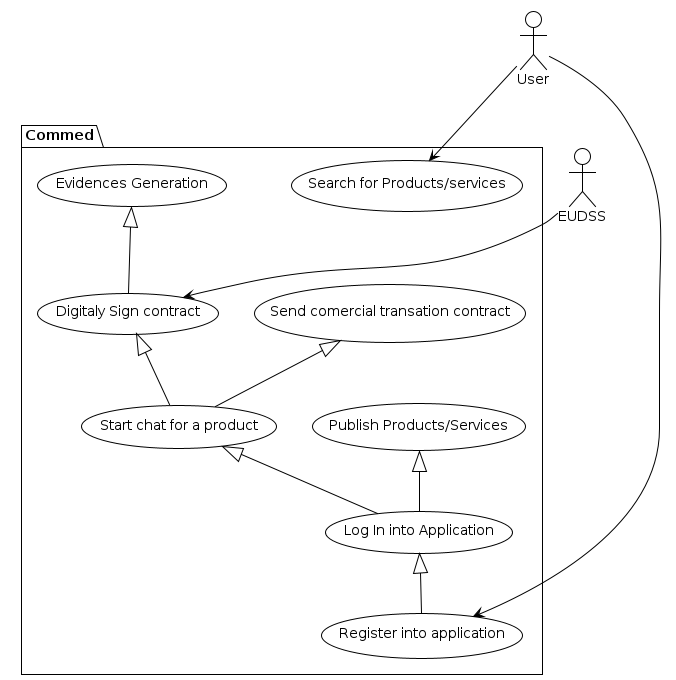
\includegraphics[width=\linewidth]{use_case_diagram/usecase_diagram.png} %TODO Update with new Use Cases file at ./use_case_diagram
\caption{Use case diagram of the application.}
\end{figure}

\subsection{Sprint 1}
\begin{itemize}

\item
  \textbf{Register into application}

  \begin{itemize}
  
  \item
    \textbf{Actors:} User
  \item
    \textbf{Purpose:} Let a user register into the application system
  \item
    \textbf{Description:} Provides a screen with a form in which the
    user is able to fulfill it and send the information to the system in
    order to be registered.
  \end{itemize}
\item
  \textbf{Log In into Application}

  \begin{itemize}
  
  \item
    \textbf{Actors:} User
  \item
    \textbf{Purpose:} Log in to the application to be able to use some
    of the application services.
  \item
    \textbf{Description:} Provides a screen with a form in which the
    user will put its email and password. Then, they will log into the
    application so that they can start using the services that it provides.
  \end{itemize}
\item
  \textbf{Search for Products/services}

  \begin{itemize}
  
  \item
    \textbf{Actors:} User
  \item
    \textbf{Purpose:} Search for any product or service the user is
    interested in.
  \item
    \textbf{Description:} Provides a searcher for every user so that
    they can look up the products or services that they are interested
    in.
  \end{itemize}
\item
  \textbf{Publish Products/Services}

  \begin{itemize}
  
  \item
    \textbf{Actors:} User
  \item
    \textbf{Purpose:} Publish services or products in order to be sold
    to other users.
  \item
    \textbf{Description:} Lets a logged user publish the products and
    services that they offer in order for them to be sold to other
    interested users.
  \end{itemize}
\item
  \textbf{Start chat for a product}

  \begin{itemize}
  
  \item
    \textbf{Actors:} User
  \item
    \textbf{Purpose:} Users can start a chat when they are interested in
    a product
  \item
    \textbf{Description:} Lets a logged user start a chat with the
    owners of either a product or a service that they are interested in,
    so that they can start a negotiation.
  \end{itemize}
\item
  \textbf{Send commercial transaction contract}

  \begin{itemize}
  
  \item
    \textbf{Actors:} User
  \item
    \textbf{Purpose:} Send a formal offer with a commercial transaction
    contract.
  \item
    \textbf{Description:} Lets the owners of given products or services
    send a formal offer containing a compliant commercial transaction
    contract within the chat in which the negotiations are taking place.
  \end{itemize}
\item
  \textbf{Digitally Sign contract}

  \begin{itemize}
  
  \item
    \textbf{Actors:} User EUSSD
  \item
    \textbf{Purpose:} Sign a commercial transaction contract sent within
    a Formal Offer.
  \item
    \textbf{Description:} Lets the users of the application sign
    digitally the contract that was sent as a Formal Offer in the chat
    in which the negotiations took place.
  \end{itemize}
\item
  \textbf{Evidences Generation}

  \begin{itemize}
  
  \item
    \textbf{Actors:} User
  \item
    \textbf{Purpose:} Provide users with evidences and the billing of a
    business transaction
  \item
    \textbf{Description:} The system will generate for both parts the
    commercial transaction with all the evidences and the billing of
    the contract.
  \end{itemize}
\end{itemize}

\subsection{Sprint 2}
%TODO: Add new Sprint 2 Use Cases Here

\hypertarget{general-architecture}{%
\section{General architecture}\label{general-architecture}}

\begin{figure}[H]
\centering
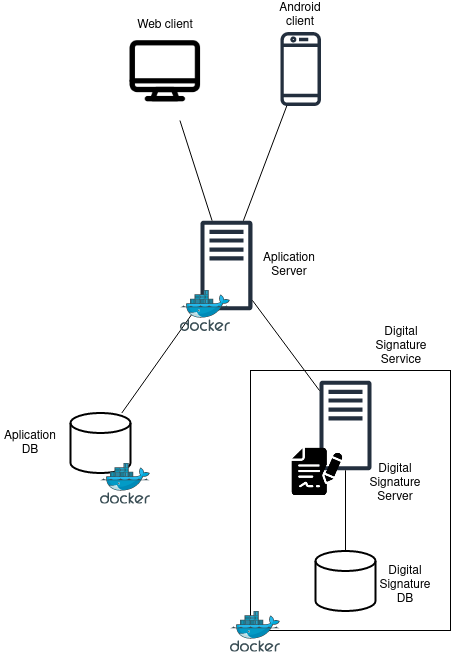
\includegraphics[width=0.6\textwidth]{architecture_diagram/Architecture.drawio.png}
\caption{General architecture of the application.}
\end{figure}

\subfile{mobile.tex} % TODO Add in these files
\subfile{frontend.tex} % TODO Add in these files - Done to review

\section{Database model}
The database model can be seen at figure \ref{fig:model-uml}.

\begin{figure}[H]
\centering
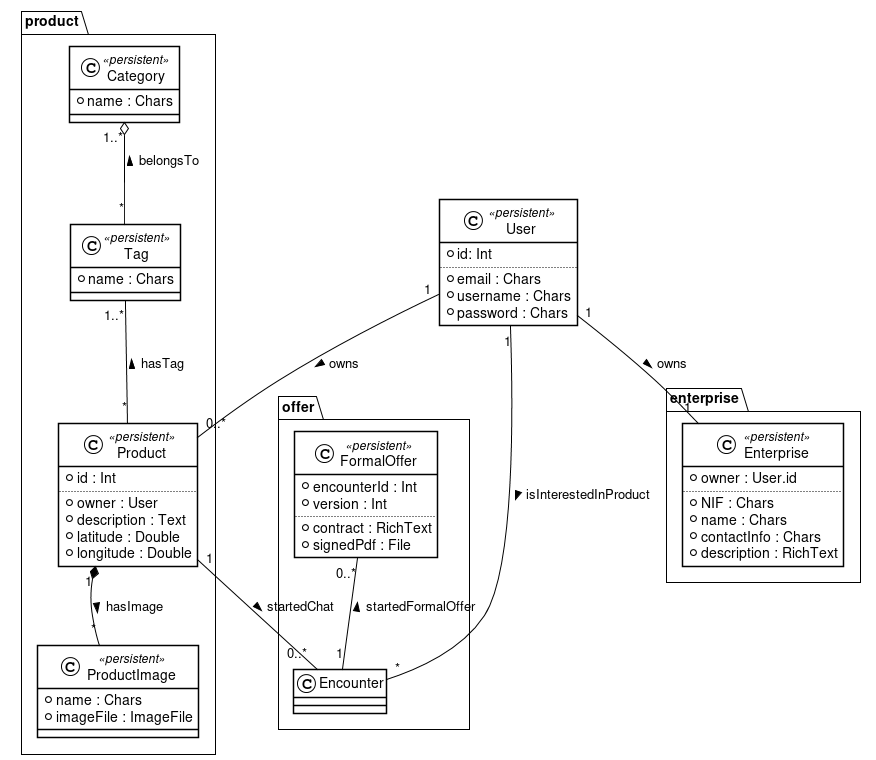
\includegraphics[width=\linewidth]{img/database-model.png}
\caption{UML diagram of the models.}
\label{fig:model-uml}
\end{figure}

\subsection{Modifications on the models}
%TODO: Explain the modifications that we did in The model.

\section{Main Screens} \label{sec:views}

\subsection{Mobile Application}
%TODO: Mobile Application screens.
\subsubsection{Wireframe}
It can be seen in the next images the main screens of the wireframe. At first, it can be seen a list of product
as the main page of the application, in the image \ref{fig:wire-1}. The next image \ref{fig:wire-2} contains the login screen, which can be accessed by clicking on the user icon the image before. The register \ref{fig:wire-3} is accessed by clicking at the sign-up option.\\
\\
The image \ref{fig:wire-4} contains the list of chats that you currently have for every product or service, and the \ref{fig:wire-5} has the detail of a particular chat, that can be seen when clicking in a item from the list of chats. The next image contains the list of formal offers \ref{fig:wire-6}. Both lists can be accessed when clicking on the icon in the bottom menu if the application.\\
\\
The last two images contains the detail of an enterprise \ref{fig:wire-7} and a submenu for things related to the user \ref{fig:wire-8}. The first image can be accessed when clicking the logo of an enterprise, and the last one can be seen when clicking on the user logo. 
\begin{figure}[H]
	\centering
	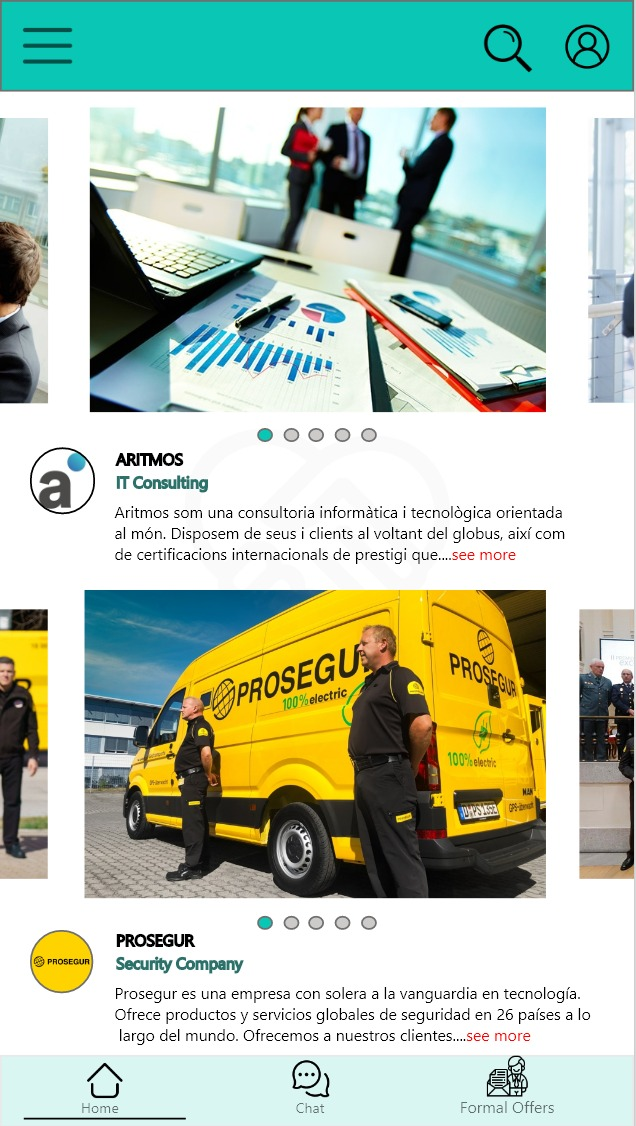
\includegraphics[width=0.5\linewidth]{img/home-page.jpeg}
	\caption{Home mobile screen, it lists the products}
	\label{fig:wire-1}
\end{figure}

\begin{figure}[H]
	\centering
	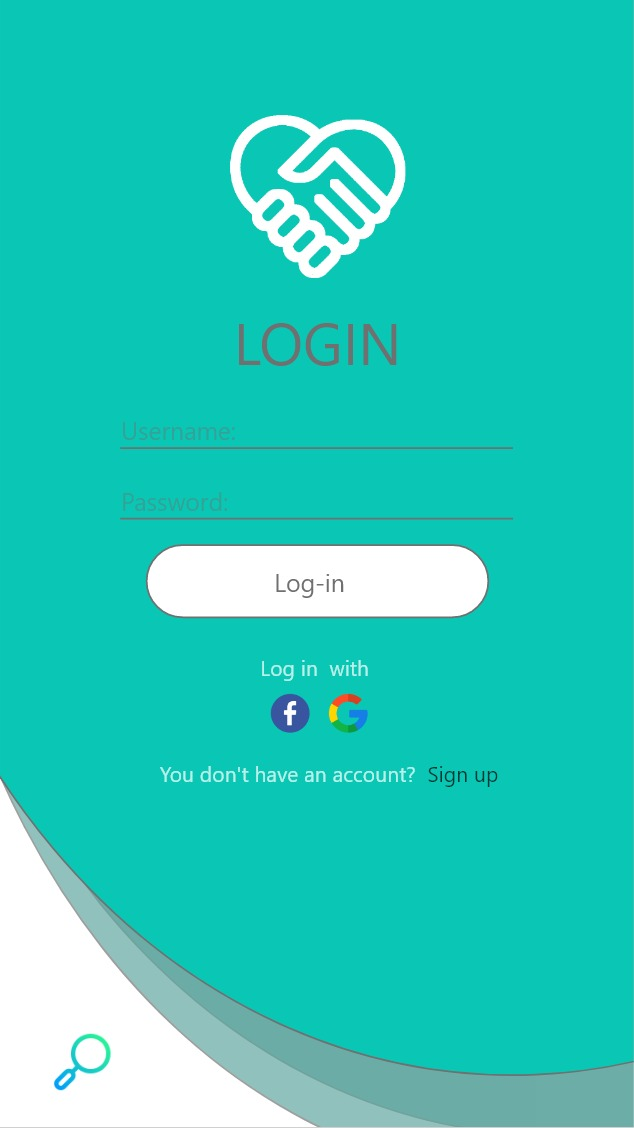
\includegraphics[width=0.5\linewidth]{img/login-page.jpeg}
	\caption{Login view}
\label{fig:wire-2}
\end{figure}

\begin{figure}[H]
	\centering
	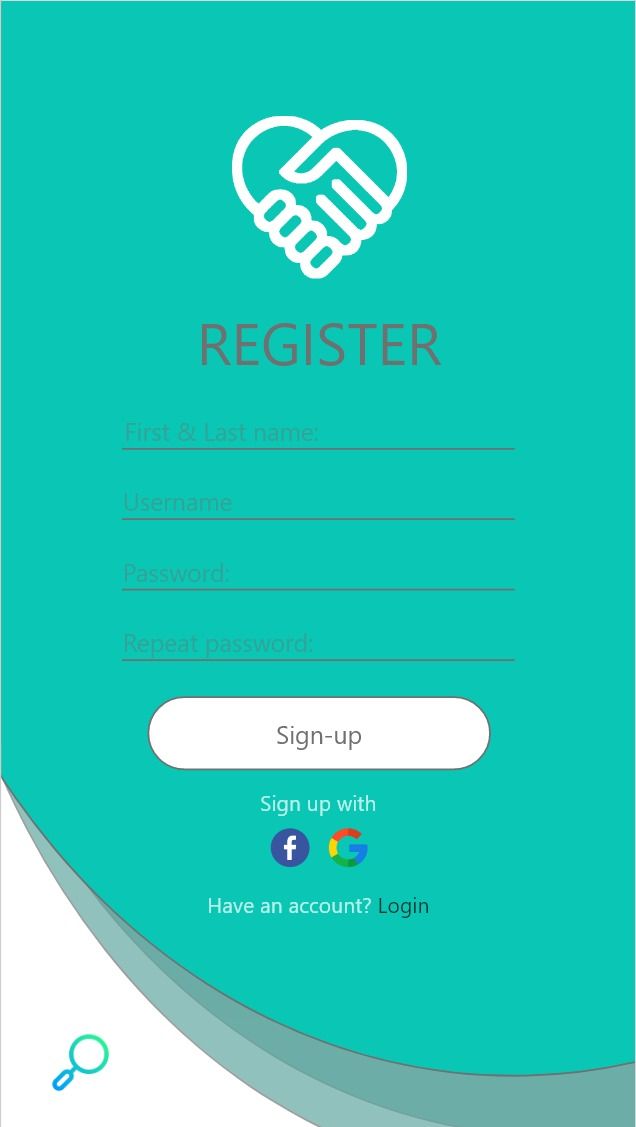
\includegraphics[width=0.5\linewidth]{img/register-page.jpeg}
	\caption{Register view}
	\label{fig:wire-3}
\end{figure}

\begin{figure}[H]
	\centering
	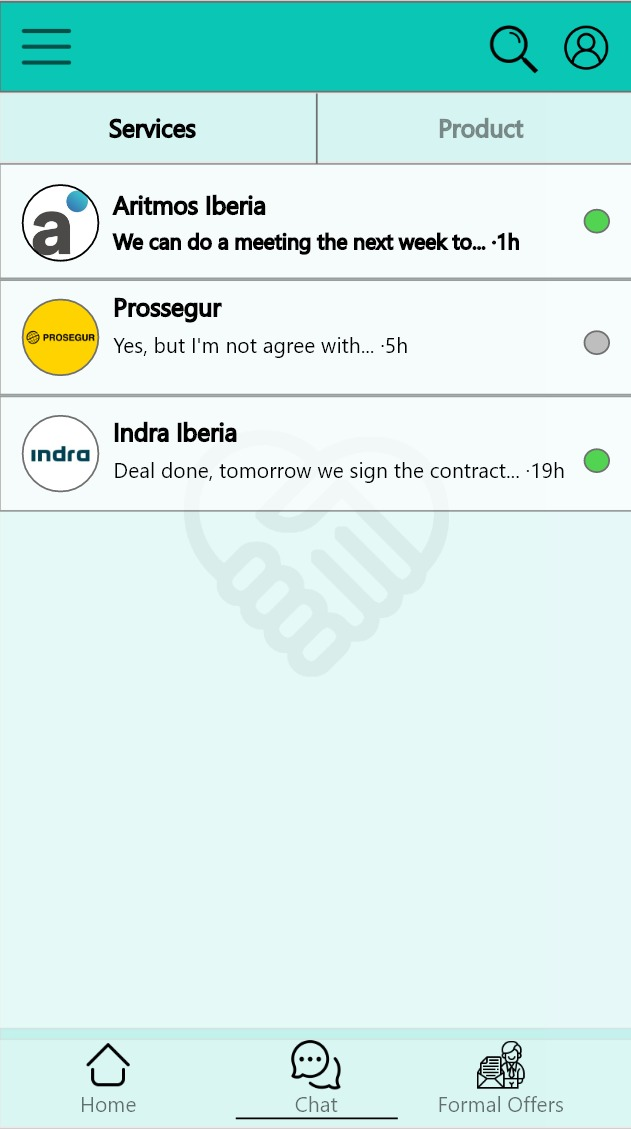
\includegraphics[width=0.5\linewidth]{img/chat-list.jpeg}
	\caption{List of the current chats.}
	\label{fig:wire-4}
\end{figure}

\begin{figure}[H]
	\centering
	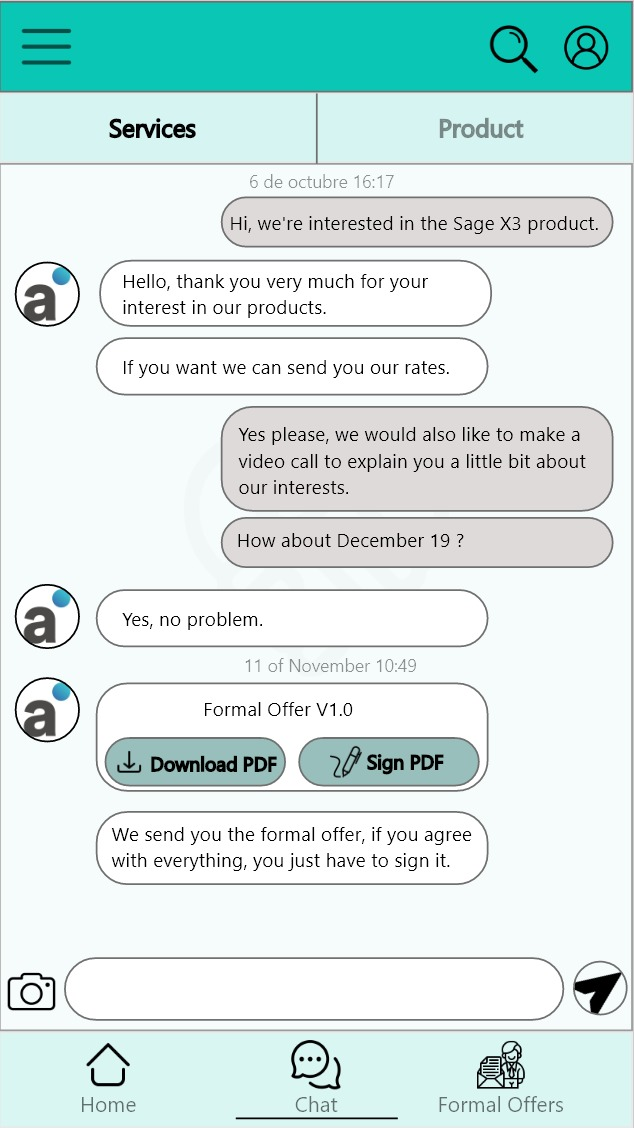
\includegraphics[width=0.5\linewidth]{img/chat-conversation.jpeg}
	\caption{A chat conversation.}
	\label{fig:wire-5}
\end{figure}

\begin{figure}[H]
	\centering
	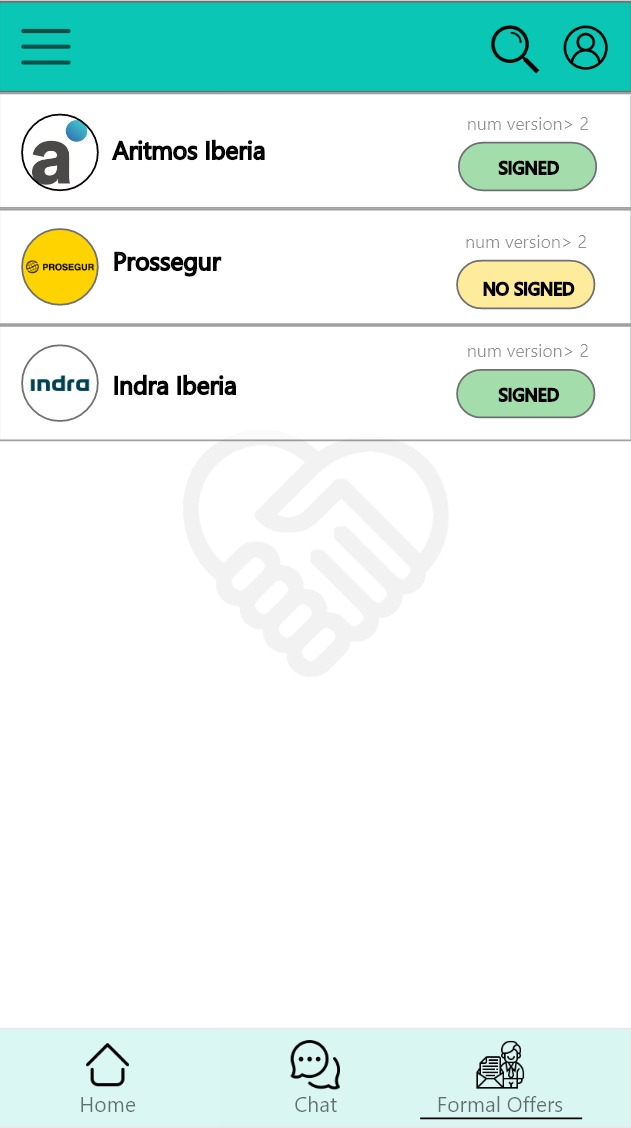
\includegraphics[width=0.5\linewidth]{img/formal-offers.jpeg}
	\caption{List of formal offers.}
	\label{fig:wire-6}
\end{figure}

\begin{figure}[H]
	\centering
	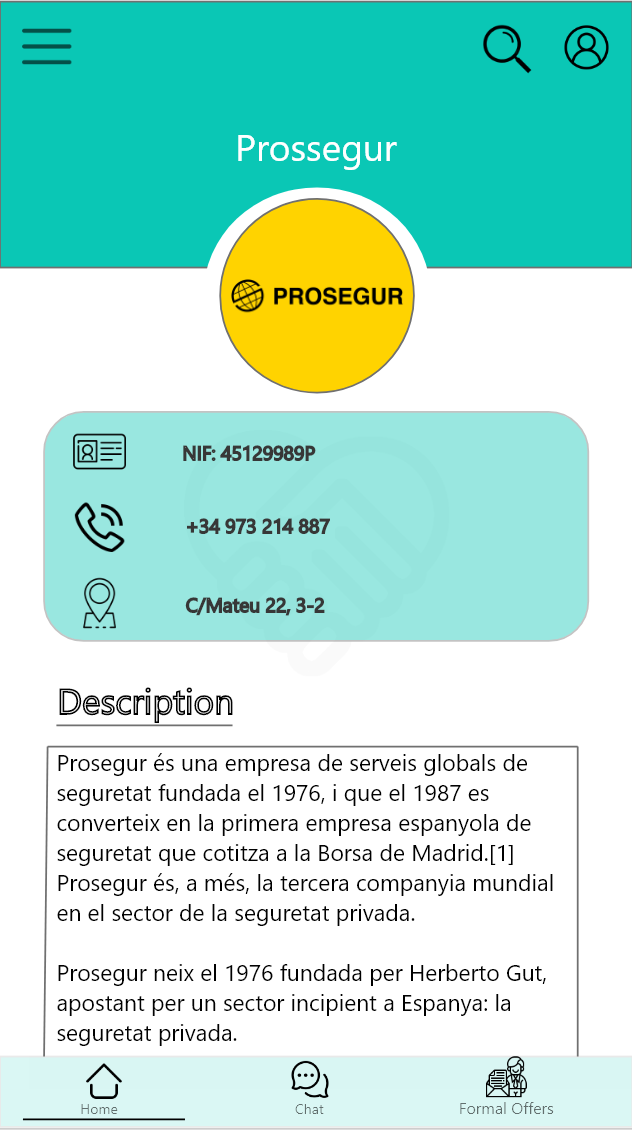
\includegraphics[width=0.5\linewidth]{img/enterprise-profile.png}
	\caption{An enterprise profile.}
	\label{fig:wire-7}
\end{figure}

\begin{figure}[H]
	\centering
	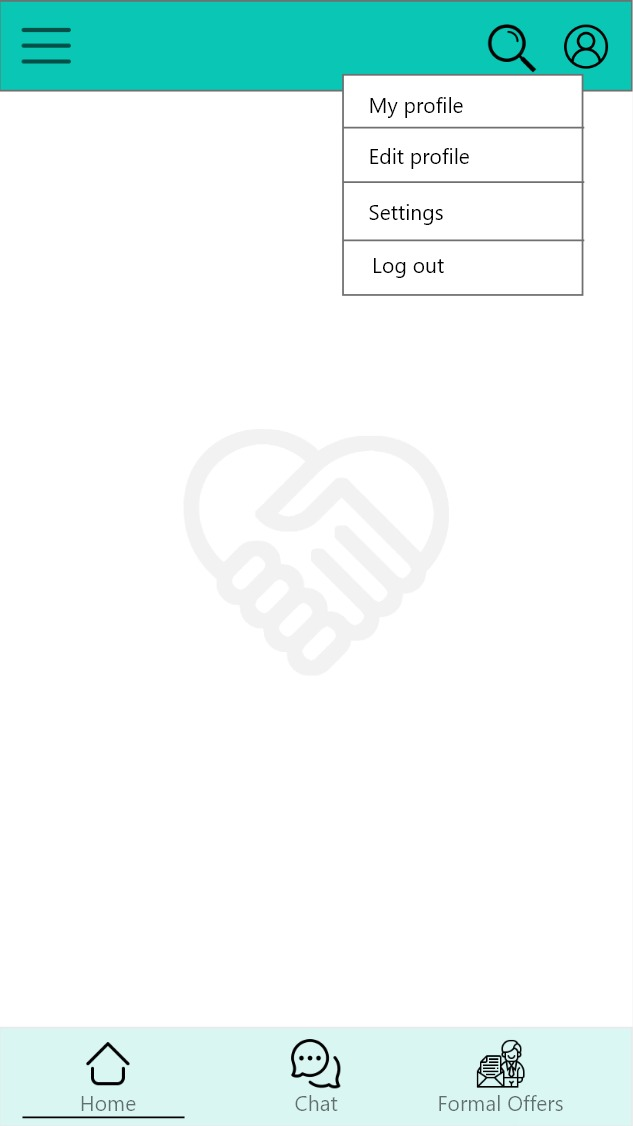
\includegraphics[width=0.5\linewidth]{img/menu-profile.jpeg}
	\caption{Menu Profile.}
	\label{fig:wire-8}
\end{figure}


\subsubsection{Application}
In this section, you will encounter all the screens that the application has currently. The first three images correspond to the home, which lists some products, the list of chats, and the list of formal offers. This can be accessed when clicking at the bottom view. It can not be slides, as it was found confusing when using the images' carousel.\\
\\
The next page \ref{fig:mobile-screen-5} is the profile of an enterprise, which is triggered when clicking a logo of the enterprise, in the pages before. In the figure \ref{fig:mobile-screen-4}, the chat between two users can be seen. It also can be seen a formal offer version, and although a formal offer version can only be send by the owner of the product, it was though that showcasing both items in the mock would be better. The next image \ref{fig:mobile-screen-3} is the searcher of the app, that can be triggered when clicking the magnifying  glass icon. It has the history of the items searched, which can be deleted when clicking the trash button, or replicated when clicking the text.\\
\\
Finally, in the images \ref{fig:mobile-screen-2}, \ref{fig:mobile-screen-1}, it is shown the registration and the login screens.
\begin{figure}[H]
	\centering
	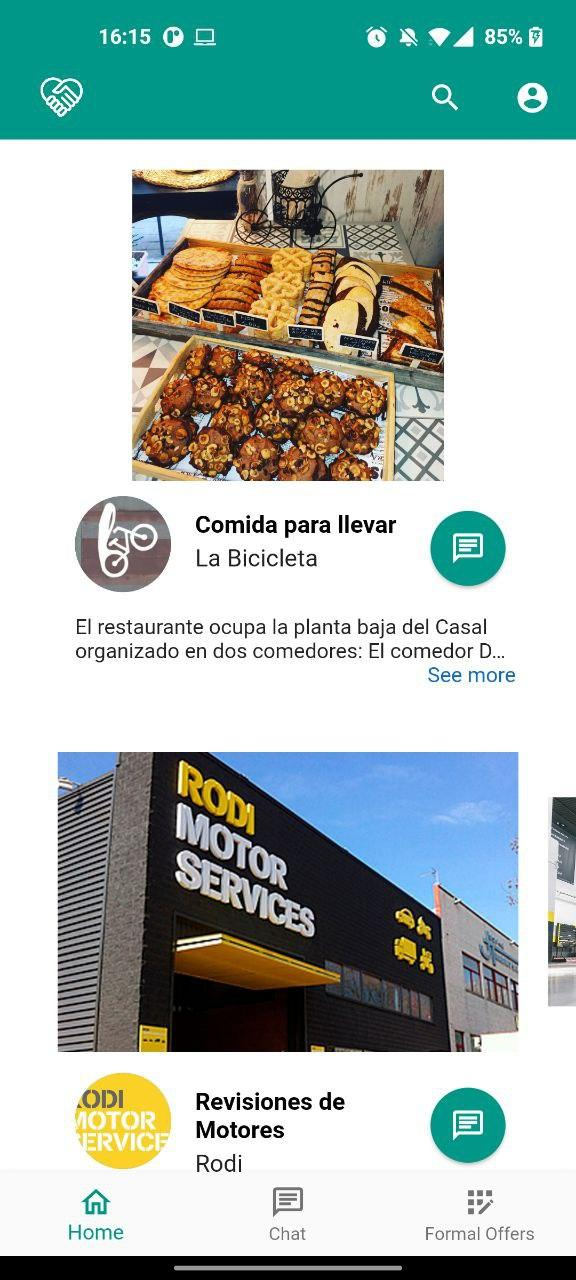
\includegraphics[width=0.5\linewidth]{img/mobile-screen-8.jpg}
	\caption{Home mobile screen, it lists the products}
	\label{fig:mobile-screen-8}
\end{figure}
\begin{figure}[H]
\centering
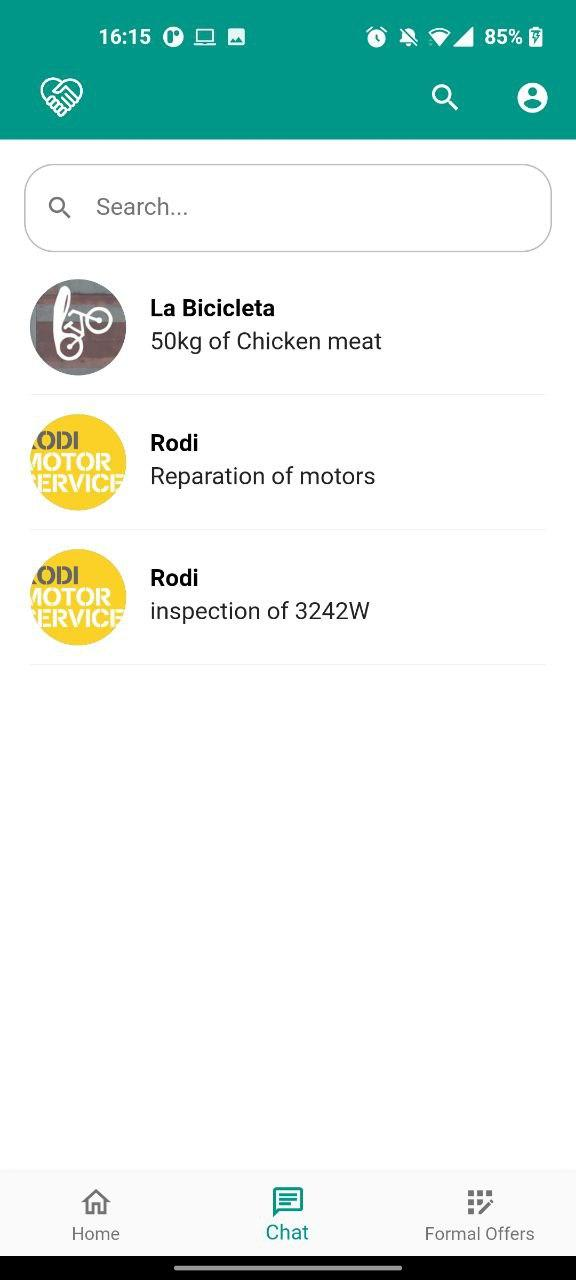
\includegraphics[width=0.5\linewidth]{img/mobile-screen-7.jpg}
\caption{List of the current chats.}
\label{fig:mobile-screen-7}
\end{figure}
\begin{figure}[H]
\centering
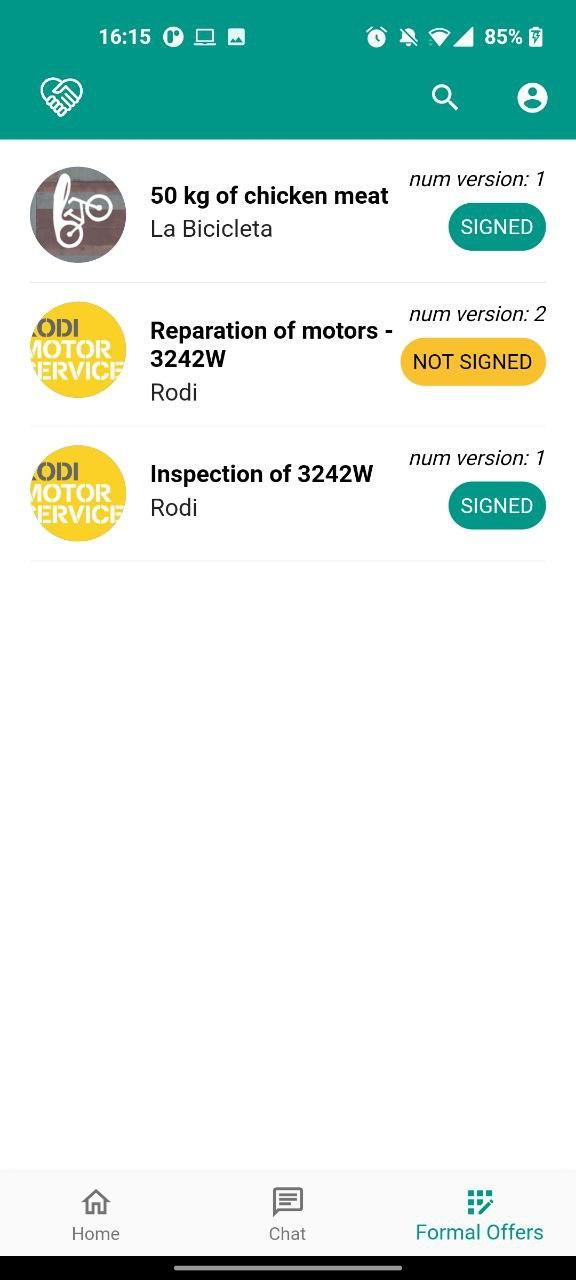
\includegraphics[width=0.5\linewidth]{img/mobile-screen-6.jpg}
\caption{List of the current formal offers.}
\label{fig:mobile-screen-6}
\end{figure}
\begin{figure}[H]
\centering
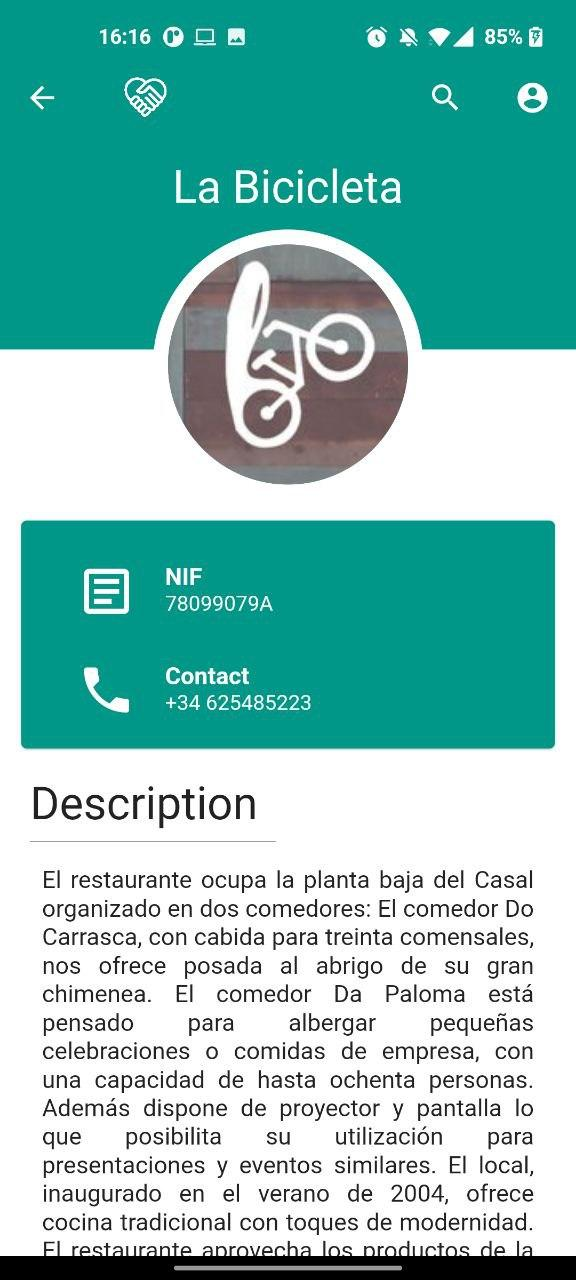
\includegraphics[width=0.5\linewidth]{img/mobile-screen-5.jpg}
\caption{Detail of an enterprise, it can be found when clicking the logo of it.}
\label{fig:mobile-screen-5}
\end{figure}
\begin{figure}[H]
\centering
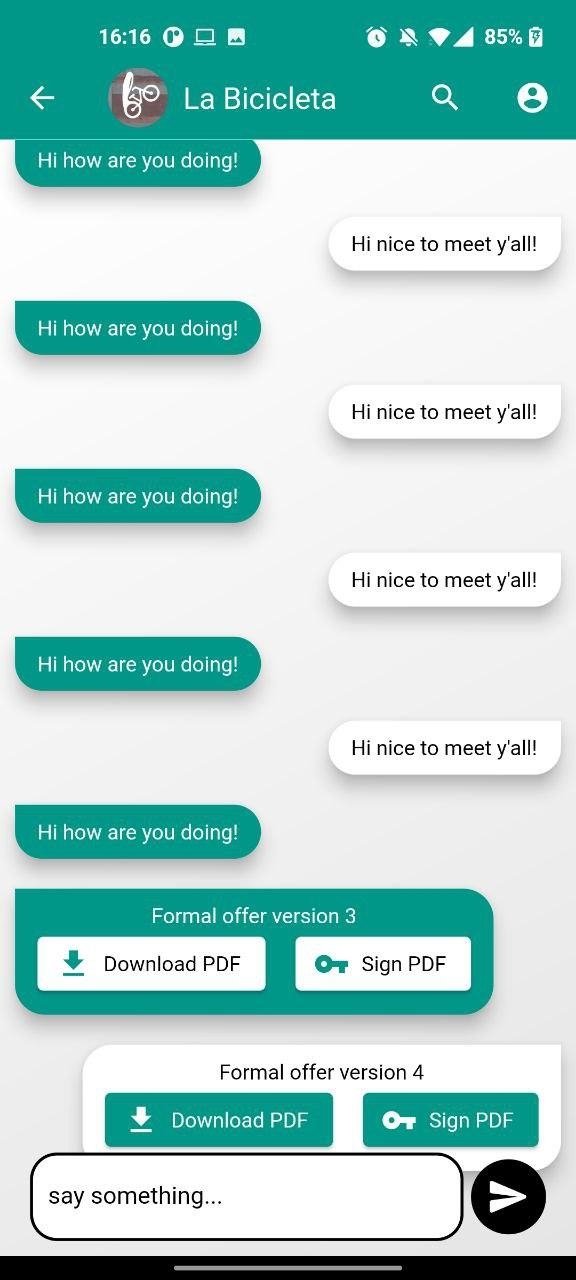
\includegraphics[width=0.5\linewidth]{img/mobile-screen-4.jpg}
\caption{Chat screen.}
\label{fig:mobile-screen-4}
\end{figure}
\begin{figure}[H]
\centering
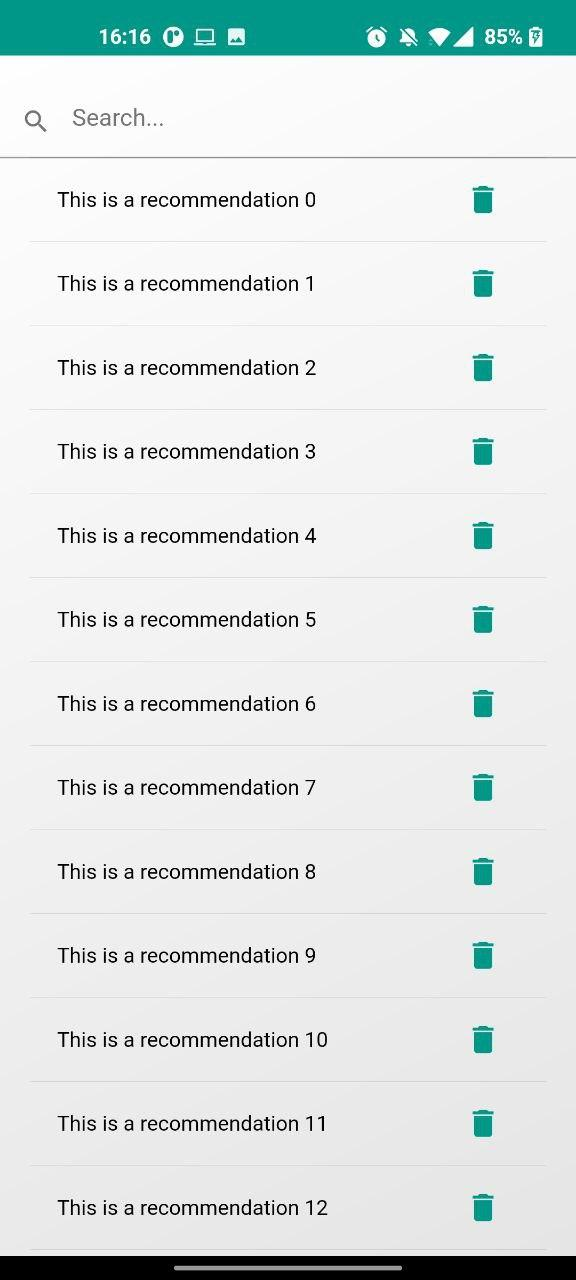
\includegraphics[width=0.5\linewidth]{img/mobile-screen-3.jpg}
\caption{Recommendations screen.}
\label{fig:mobile-screen-3}
\end{figure}
\begin{figure}[H]
\centering
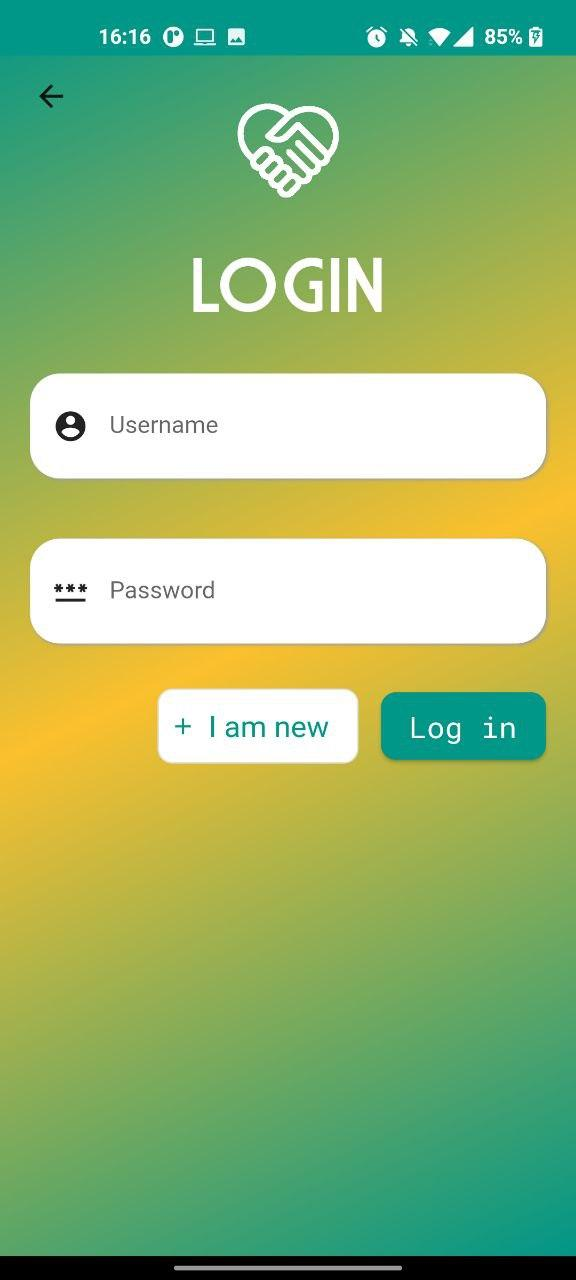
\includegraphics[width=0.5\linewidth]{img/mobile-screen-2.jpg}
\caption{Login view.}
\label{fig:mobile-screen-2}
\end{figure}
\begin{figure}[H]
\centering
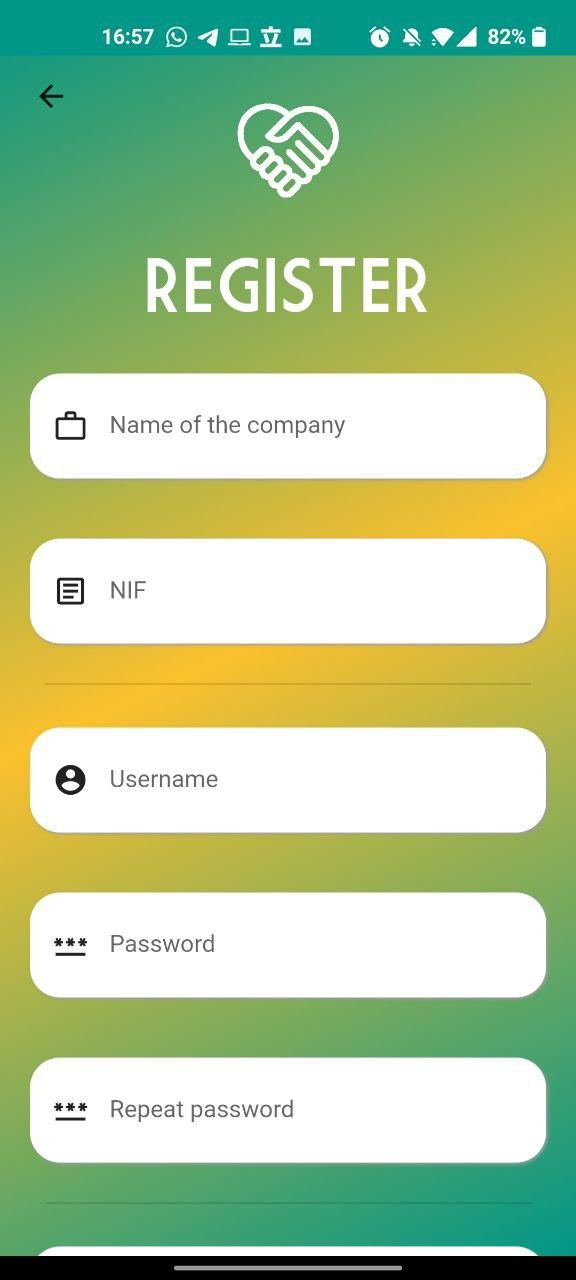
\includegraphics[width=0.5\linewidth]{img/mobile-screen-1.jpg}
\caption{Registration screen.}
\label{fig:mobile-screen-1}
\end{figure}


\subsection{Web Client}
%TODO: Web Client Screens.

\end{document}
